\section{Padrão de Projeto \textit{Model-View-Controller}}

O MVC é um padrão de projeto que é considerado como um dos mais importantes na área da ciência da computação, pois este pode ser interpretado como algo mais próximo de uma filosofia de desenvolvimento de arquitetura de código, do que de um padrão de projeto que resolve instâncias de problemas de um domínio específico. O MVC possui uma grande abertura de interpretação e aplicação, podendo ser adotado desde subsistemas até aplicações inteiras. Essencialmente, o MVC é definido em três entidades: a \textit{model}, a \textit{view}, e a \textit{controller} \cite{Bucanek2009}.

As próximas subseções tem como objetivo descrever cada uma dessas entidades e qual papel desempenham dentro do contexto do padrão de projeto MVC.

\subsection{\textit{Model}}

A \textit{model} é a entidade do MVC que possui como preocupação encapsular informações do domínio do problema a ser resolvido pela aplicação. Um objeto de dados \textit{model} deve saber guardar, encapsular e abstrair os dados. Vale observar também que cada entidade idealmente não deve extrapolar suas funções, portanto, uma \textit{model} deve saber serializar seus dados, mas não deve saber como implementar uma funcionalidade de "salvar como" \cite{Bucanek2009}.

\subsection{\textit{View}}

Em poucas palavras, a \textit{view} é a entidade do MVC que apresenta informações na tela para o usuário final. Porém, a \textit{view} desempenha muitos outros papeis; na verdade, ela é a ponte entre o usuário e o sistema. Dessa forma, a \textit{view} é responsável por captar o \textit{input} do usuário e transformá-lo em comandos para o sistema processar. Outro aspecto importante é o escopo que uma \textit{view} pode atuar. No desenvolvimento de aplicações com o modelo MVC, objetos de \textit{view} podem ser generalistas ao ponto de apenas saberem renderizar e lidar com textos, imagens e mídias, ou podem ser específicos ao ponto de saber renderizar apenas objetos específicos do sistema definidos no código pelo programador \cite{Bucanek2009}.

\subsection{\textit{Controller}}

A \textit{controller} é a entidade do MVC que implementa as ações do sistema. Como já mencionado, as \textit{models} sabem gerenciar seus dados a nível de persistência e abstração, as \textit{views} são responsáveis por coletar o \textit{input} do usuário para disparar as ações, estas que residem nas \textit{controllers}. Uma ação realizada por uma \textit{controller}, por exemplo, seria o comando "salvar como" de um dado armazenado dentro de uma \textit{model} \cite{Bucanek2009}.
Em geral, a comunicação realizada pelas entidades no modelo MVC pode ser visualizada na Figura \ref{fig:diagrama_mvc}.  

\begin{figure}
    \centering
    \caption{Comunicação entre as entidades do MVC}
    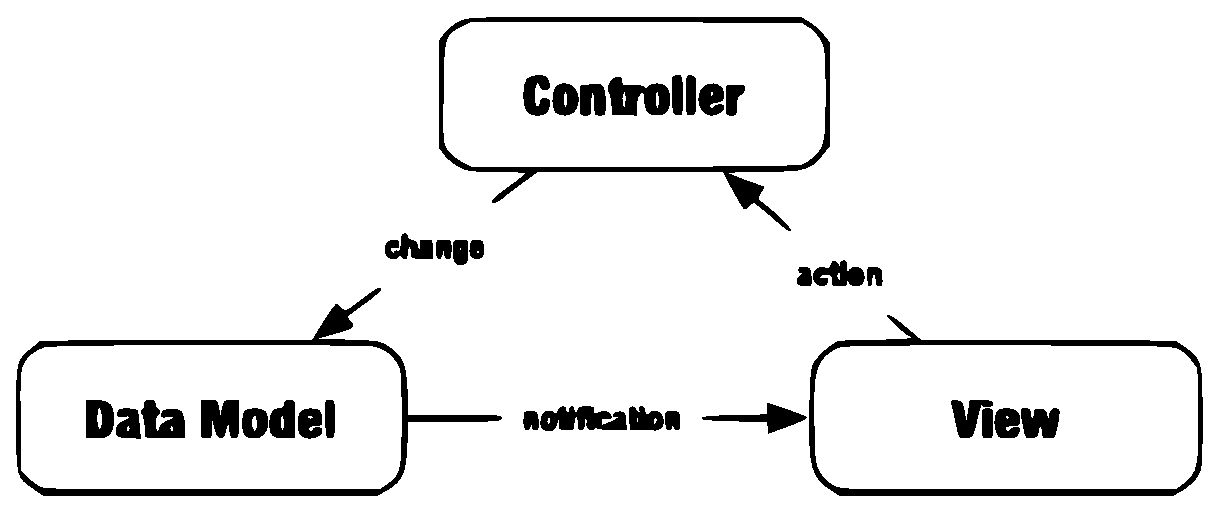
\includegraphics[width=\textwidth]{figuras/diagrama_mvc.eps}
    \fonte{\cite{Bucanek2009}}
    \label{fig:diagrama_mvc}
\end{figure}